% =====================================================================
% Toán 7 · Bài 9. Hai đường thẳng song song và dấu hiệu nhận biết (KNTT)
% Khối lý thuyết theo CÚ PHÁP BÀI GIẢNG MỚI (docs/bai-giang/cu-phap.md).
% Thầy Linh duyệt kịch bản 26/11/2026 qua bản thử docs/bai-giang/ban-thu-bai9.html.
% Dùng làm: (1) dữ liệu kiểm tra cho bộ đọc và giao diện (tests), (2) bài mẫu cho người soạn.
% Khi nạp lên app: chỉ thay khối \begin{lythuyet}…\end{lythuyet} của chủ đề
% lop7-b9-goc-o-vi-tri-dac-biet-tia-phan-giac-cua-mot-goc; GIỮ NGUYÊN phần \man{…} câu hỏi.
% Đánh số góc theo SGK Hình 3.16 cho cả bài: tại mỗi giao điểm
%   trên-trái 2, trên-phải 3, dưới-trái 1, dưới-phải 4.
% =====================================================================
\begin{lythuyet}

% ---------------- MỞ ĐẦU ----------------
\begin{modau}
\cherry{Người thợ đặt ê ke vào chỗ các thanh ngang gặp thanh dọc. Em đặt thử nhé!}
\cauhoi{Vì sao chỉ cần như vậy là đủ biết các thanh ngang song song?}
\nutbuoc{Đặt ê ke}
\begin{hinhbuoc}
\begin{tikzpicture}[line cap=round]
\fill[orange!12] (-3.2,0) -- (0,4) -- (3.2,0) -- cycle;
\draw[brown!70!black, line width=3pt, line join=round] (-3.2,0) -- (0,4) -- (3.2,0);
\fill[brown!70!black] (-3.3,-0.35) rectangle (3.3,0);
\draw[brown!80!black, line width=3.5pt] (-2.5,0.9) -- (2.5,0.9);
\draw[brown!80!black, line width=3.5pt] (-1.75,1.9) -- (1.75,1.9);
\draw[brown!80!black, line width=3.5pt] (-1,2.9) -- (1,2.9);
\draw[brown!60!black, line width=4pt] (0,0.05) -- (0,3.9);
\node[font=\small, text=brown!50!black, right] at (0.1,3.55) {thanh dọc};
\node[font=\small, text=brown!50!black] at (-1.6,1.4) {thanh ngang};
\hien{2}{\draw[red, line width=1.2pt] (0.3,0.9) -- (0.3,1.2) -- (0,1.2);}
\hien{3}{\draw[red, line width=1.2pt] (0.3,1.9) -- (0.3,2.2) -- (0,2.2);}
\hien{4}{\draw[red, line width=1.2pt] (0.3,2.9) -- (0.3,3.2) -- (0,3.2);}
\phu{2}{2}{\draw[orange!80!black, fill=orange!35, line width=1pt] (0.05,0.95) -- (0.85,0.95) -- (0.05,1.75) -- cycle;}
\phu{3}{3}{\draw[orange!80!black, fill=orange!35, line width=1pt] (0.05,1.95) -- (0.85,1.95) -- (0.05,2.75) -- cycle;}
\phu{4}{4}{\draw[orange!80!black, fill=orange!35, line width=1pt] (0.05,2.95) -- (0.65,2.95) -- (0.05,3.55) -- cycle;}
\end{tikzpicture}
\loibuoc{Khung mái nhà có một thanh dọc và ba thanh ngang.}
\loibuoc{Thanh ngang thứ nhất vuông góc với thanh dọc.}
\loibuoc{Thanh ngang thứ hai cũng vuông góc với thanh dọc.}
\loibuoc{Cả ba thanh ngang đều vuông góc với thanh dọc. Học xong bài này, em sẽ tự giải thích được!}
\end{hinhbuoc}
\end{modau}

% ---------------- PHẦN 1 ----------------
\phan{Góc so le trong, góc đồng vị}{Nhận biết các góc tạo bởi một đường thẳng cắt hai đường thẳng}
\nhaclai{Đường thẳng $c$ cắt $a$, $b$ tại $A$, $B$. \\ \textbf{So le trong}: nằm giữa $a$, $b$ và ở hai phía của $c$: $\widehat{A_1}$ và $\widehat{B_3}$; $\widehat{A_4}$ và $\widehat{B_2}$. \\ \textbf{Đồng vị}: cùng vị trí ở hai đỉnh: $\widehat{A_1}$ và $\widehat{B_1}$; $\widehat{A_2}$ và $\widehat{B_2}$; $\widehat{A_3}$ và $\widehat{B_3}$; $\widehat{A_4}$ và $\widehat{B_4}$.}
\hinhchung{\hinhmau{cat-tuyen}{duong=a,b,c; diem=A,B}}

\cherry{Đường thẳng $c$ cắt $a$ tại $A$ và cắt $b$ tại $B$.}
\trangthai{so=an}
\thungay{Tại hai điểm $A$ và $B$ có tất cả bao nhiêu góc?}{8 góc}{4 góc}{Đúng! Mỗi đỉnh có 4 góc. Ta đánh số chúng 1, 2, 3, 4 như trên hình.}{Mỗi điểm $A$, $B$ có 4 góc, nên có tất cả 8 góc.}
\saukhitra{so=hien}

\chamvung{Chạm vào phần nằm \textbf{giữa} hai đường thẳng $a$ và $b$.}{giua}{Đúng rồi! Các góc nằm trong phần tô vàng là các góc nằm \textbf{giữa} $a$ và $b$.}

\trangthai{vung=giua; to=A1:cam,B3:cam,A4:lam,B2:lam}
\dinhnghia{Cặp góc so le trong}{Hai góc nằm \textbf{giữa} $a$, $b$ và ở \textbf{hai phía} của $c$ gọi là một cặp góc \textbf{so le trong}: \\ $\widehat{A_1}$ và $\widehat{B_3}$; $\widehat{A_4}$ và $\widehat{B_2}$.}

\cherry{Chạm vào góc so le trong với $\widehat{A_4}$.}
\trangthai{to=A4:cam}
\chamhinh{Chạm vào góc so le trong với $\widehat{A_4}$.}{B2}{Đúng! $\widehat{A_4}$ và $\widehat{B_2}$ cùng nằm giữa $a$, $b$ và ở hai phía của $c$.}{Góc cần tìm ở đỉnh $B$.}
\nhac{B3}{$\widehat{B_3}$ cùng phía (bên phải $c$) với $\widehat{A_4}$. Hãy tìm ở phía bên kia.}
\nhac{B1}{$\widehat{B_1}$ nằm ngoài phần giữa $a$ và $b$.}
\nhac{B4}{$\widehat{B_4}$ nằm ngoài phần giữa $a$ và $b$.}

\cherry{Trượt bốn góc ở đỉnh $A$ dọc theo $c$ xuống đỉnh $B$. Góc nào trùng chỗ góc nào?}
\truot{Trượt xuống $B$}{$\widehat{A_1}$ trùng chỗ $\widehat{B_1}$, $\widehat{A_2}$ trùng chỗ $\widehat{B_2}$, $\widehat{A_3}$ trùng chỗ $\widehat{B_3}$, $\widehat{A_4}$ trùng chỗ $\widehat{B_4}$. \\ Hai góc ở \textbf{vị trí giống nhau} như vậy gọi là một cặp góc \textbf{đồng vị}.}

\trangthai{to=A1:cam,B1:cam,A2:lam,B2:lam,A3:luc,B3:luc,A4:tim,B4:tim}
\dinhnghia{Cặp góc đồng vị}{Bốn cặp góc \textbf{đồng vị} (cùng màu trên hình): \\ $\widehat{A_1}$ và $\widehat{B_1}$; $\widehat{A_2}$ và $\widehat{B_2}$; \\ $\widehat{A_3}$ và $\widehat{B_3}$; $\widehat{A_4}$ và $\widehat{B_4}$.}

\cherry{Chạm vào góc đồng vị với $\widehat{A_3}$.}
\trangthai{to=A3:cam}
\chamhinh{Chạm vào góc đồng vị với $\widehat{A_3}$.}{B3}{Chính xác! $\widehat{A_3}$ và $\widehat{B_3}$ cùng ở trên-phải tại mỗi đỉnh.}{Góc cần tìm ở đỉnh $B$.}
\nhac{B1}{$\widehat{B_1}$ ở dưới-trái, còn $\widehat{A_3}$ ở trên-phải.}
\nhac{B2}{$\widehat{B_2}$ ở bên trái $c$, còn $\widehat{A_3}$ ở bên phải.}
\nhac{B4}{$\widehat{B_4}$ ở dưới $b$, còn $\widehat{A_3}$ ở trên $a$.}

\cherry{Thử với một hình mới nhé!}
\hinhrieng{\hinhmau{cat-tuyen}{duong=x-y,u-v,m-n; diem=P,Q; c=phai}}
\trangthai{so=an; to=P1:cam}
\thungay{Đường thẳng $mn$ cắt $xy$ tại $P$, cắt $uv$ tại $Q$. Góc nào so le trong với $\widehat{xPQ}$?}{$\widehat{PQv}$}{$\widehat{PQu}$}{Đúng! $\widehat{xPQ}$ và $\widehat{PQv}$ nằm giữa $xy$, $uv$ và ở hai phía của $mn$.}{$\widehat{PQu}$ và $\widehat{xPQ}$ cùng ở bên trái $mn$, không phải hai phía. Góc so le trong với $\widehat{xPQ}$ là $\widehat{PQv}$.}
\saukhitra{to=P1:cam,Q3:cam}

% ---------------- PHẦN 2 ----------------
\phan{Khi có một cặp góc so le trong bằng nhau}{Biết các góc còn lại bằng nhau thế nào}
\nhaclai{Nếu $c$ cắt $a$, $b$ và có \textbf{một cặp góc so le trong bằng nhau} thì hai góc so le trong còn lại bằng nhau và các cặp góc đồng vị bằng nhau.}
\hinhchung{\hinhmau{cat-tuyen}{duong=a,b,c; diem=A,B}}

\cherry{Biết $\widehat{A_1}=\widehat{B_3}=60^\circ$ (một cặp so le trong). Tính hai góc so le trong còn lại!}
\trangthai{to=A1:cam,B3:cam; do=A1:60°,B3:60°}
\emtinh{$\widehat{A_4}=\,?$}{$120^\circ$}{$60^\circ$}{Đúng: $\widehat{A_1}$ và $\widehat{A_4}$ kề bù nên $\widehat{A_4}=180^\circ-60^\circ=120^\circ$.}{$\widehat{A_1}$ và $\widehat{A_4}$ kề bù (tổng $180^\circ$), không bằng nhau.}{to=A4:lam; do=A4:120°}
\emtinh{$\widehat{B_2}=\,?$}{$120^\circ$}{$60^\circ$}{Đúng: $\widehat{B_3}$ và $\widehat{B_2}$ kề bù nên $\widehat{B_2}=180^\circ-60^\circ=120^\circ$.}{$\widehat{B_3}$ và $\widehat{B_2}$ kề bù, không bằng nhau.}{to=B2:lam; do=B2:120°}
\ketluan{Vậy $\widehat{A_4}=\widehat{B_2}$: hai góc so le trong còn lại \textbf{cũng bằng nhau}!}

\cherry{Còn cặp góc đồng vị thì sao? Vẫn biết $\widehat{B_3}=60^\circ$.}
\trangthai{to=A1:cam,B3:luc; do=A1:60°,B3:60°}
\emtinh{$\widehat{B_1}=\,?$}{$60^\circ$}{$120^\circ$}{Đúng: $\widehat{B_1}$ và $\widehat{B_3}$ đối đỉnh nên $\widehat{B_1}=60^\circ$.}{$\widehat{B_1}$ và $\widehat{B_3}$ là hai góc đối đỉnh nên bằng nhau.}{to=B1:cam; do=B1:60°}
\ketluan{Vậy cặp góc đồng vị $\widehat{A_1}=\widehat{B_1}$!}

\trangthai{to=A1:cam,B3:cam; do=A1:60°,A2:120°,A3:60°,A4:120°,B1:60°,B2:120°,B3:60°,B4:120°}
\tinhchat{Khi có một cặp góc so le trong bằng nhau}{Nếu $c$ cắt $a$, $b$ và có \textbf{một cặp góc so le trong bằng nhau} thì: \\ • hai góc so le trong còn lại bằng nhau; \\ • các cặp góc đồng vị bằng nhau.}

\cherry{Đổi số đo, em tự tính nhé!}
\trangthai{to=A1:cam,B3:cam; do=A1:40°,B3:40°}
\thungay{Biết $\widehat{A_1}=\widehat{B_3}=40^\circ$. Góc đồng vị với $\widehat{A_2}$ bằng bao nhiêu?}{$140^\circ$}{$40^\circ$}{Đúng: $\widehat{A_2}=180^\circ-40^\circ=140^\circ$, và góc đồng vị $\widehat{B_2}=\widehat{A_2}=140^\circ$.}{$\widehat{A_2}$ kề bù với $\widehat{A_1}$ nên $\widehat{A_2}=140^\circ$, góc đồng vị $\widehat{B_2}$ cũng bằng $140^\circ$.}
\saukhitra{to=A2:lam,B2:lam; do=A2:140°,B2:140°}

% ---------------- PHẦN 3 ----------------
\phan{Dấu hiệu nhận biết hai đường thẳng song song}{Dùng cặp góc so le trong, đồng vị để biết hai đường thẳng song song}
\nhaclai{Nếu $c$ cắt hai đường thẳng phân biệt $a$, $b$ và có \textbf{một cặp góc so le trong bằng nhau} hoặc \textbf{một cặp góc đồng vị bằng nhau} thì $a\parallel b$. \\ Hai đường thẳng phân biệt cùng vuông góc với một đường thẳng thứ ba thì song song.}

\cherry{Muốn biết $c$ và $d$ có điểm chung không, phải kéo dài chúng ra ngoài trang giấy!}
\hinhrieng{\begin{hinhbuoc}
\begin{tikzpicture}[line cap=round]
\draw[line width=1pt] (0,-1.3) -- (0,3.5) node[above right] {$u$};
\draw[line width=1pt] (-2.8,2) -- (2.9,2) node[above right] {$d$};
\draw[line width=1pt] (-2.8,0.994) -- (2.9,-0.011) node[above right] {$c$};
\draw[line width=0.9pt] (-0.25,2) -- (-0.25,2.25) -- (0,2.25);
\fill[orange!45] (0,0.5) -- (0,1.0) arc (90:170:0.5) -- cycle;
\node[font=\small\bfseries, text=orange!80!black] at (-0.55,1.15) {$80^\circ$};
\hien{2}{\draw[line width=1pt, dashed] (-9.2,2) -- (-2.8,2);
\draw[line width=1pt, dashed] (-9.2,2.122) -- (-2.8,0.994);
\fill[red] (-8.507,2) circle (0.12);
\draw[gray, dashed] (-3.1,-1.5) rectangle (3.3,3.9);
\node[font=\small, text=gray] at (0.1,-1.25) {trang giấy};}
\path (-9.4,-1.6) rectangle (3.4,4);
\end{tikzpicture}
\loibuoc{Hai đường thẳng $c$ và $d$, đường thẳng $u$ cắt cả hai.}
\loibuoc{Thu nhỏ hình mới thấy: $c$ và $d$ cắt nhau ở rất xa (chấm đỏ), ngoài trang giấy.}
\end{hinhbuoc}}
\thungay{Có cách nào biết hai đường thẳng song song mà không cần kéo dài?}{Xét một cặp góc tạo bởi đường thẳng $u$ cắt chúng}{Không có, phải kéo dài đến khi gặp nhau}{Đúng hướng! Phần này chỉ em cách làm.}{Có cách đấy: xét một cặp góc tạo bởi $u$ cắt $c$ và $d$.}

\hinhrieng{\hinhmau{cat-tuyen}{duong=a,b,c; diem=A,B; song-song=1; c=phai}}
\trangthai{so=an}
\chuyen{Cặp so le trong}{to=A1:cam,B3:cam}{Cặp đồng vị}{to=A1:lam,B1:lam}
\dinhly{Dấu hiệu nhận biết hai đường thẳng song song}{Nếu $c$ cắt hai đường thẳng phân biệt $a$, $b$ và có \textbf{một cặp góc so le trong bằng nhau} hoặc \textbf{một cặp góc đồng vị bằng nhau} thì $a\parallel b$.}

\hinhrieng{\hinhmau{cat-tuyen}{duong=x-y,x'-y',z-z'; diem=A,B; song-song=1; c=phai}}
\trangthai{so=an; to=A1:cam,B3:cam; do=A1:70°,B3:70°}
\vidu{Quan sát hình và giải thích vì sao $xy\parallel x'y'$.}{Ta có $\widehat{xAB}=\widehat{ABy'}=70^\circ$. \\ Hai góc này ở vị trí \textbf{so le trong}. \\ Do đó $xy\parallel x'y'$ (dấu hiệu nhận biết hai đường thẳng song song).}

\cherry{Đến lượt em giải thích!}
\hinhrieng{\begin{hinhbuoc}
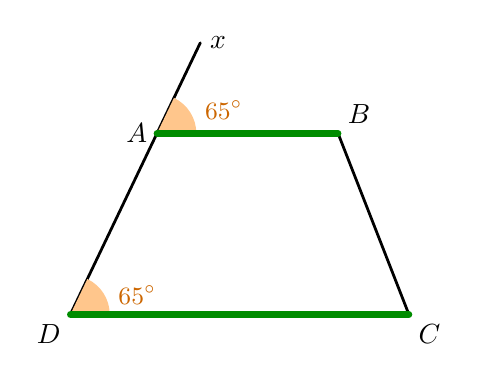
\begin{tikzpicture}[line cap=round]
\coordinate (D) at (0,0); \coordinate (C) at (4.3,0); \coordinate (A) at (1.1,2.3); \coordinate (B) at (3.4,2.3); \coordinate (X) at (1.65,3.45);
\draw[line width=1pt] (D) -- (C) -- (B) -- (A); \draw[line width=1pt] (D) -- (X);
\fill[orange!45] (A) -- ++(0:0.5) arc (0:64.4:0.5) -- cycle;
\fill[orange!45] (D) -- ++(0:0.5) arc (0:64.4:0.5) -- cycle;
\node[font=\small\bfseries, text=orange!80!black] at (1.95,2.6) {$65^\circ$};
\node[font=\small\bfseries, text=orange!80!black] at (0.85,0.25) {$65^\circ$};
\hien{2}{\draw[green!55!black, line width=2.4pt] (A) -- (B); \draw[green!55!black, line width=2.4pt] (D) -- (C);}
\node[below left] at (D) {$D$}; \node[below right] at (C) {$C$}; \node[left] at (A) {$A$}; \node[above right] at (B) {$B$}; \node[right] at (X) {$x$};
\end{tikzpicture}
\loibuoc{Tứ giác $ABCD$, tia $Ax$ nằm trên đường thẳng $DA$.}
\loibuoc{$AB\parallel DC$.}
\end{hinhbuoc}}
\thungay{Biết $\widehat{xAB}=\widehat{ADC}=65^\circ$. Vì sao $AB\parallel DC$?}{Vì có một cặp góc đồng vị bằng nhau}{Vì có một cặp góc so le trong bằng nhau}{Đúng! Đường thẳng $Dx$ cắt $AB$ và $DC$; $\widehat{xAB}$ và $\widehat{ADC}$ ở vị trí đồng vị và bằng nhau.}{$\widehat{xAB}$ và $\widehat{ADC}$ ở vị trí giống nhau (cùng phía trên-phải), nên là cặp góc \textbf{đồng vị}.}

\cherry{Hai góc vuông ở $H$ và $K$ là một cặp góc đồng vị!}
\hinhrieng{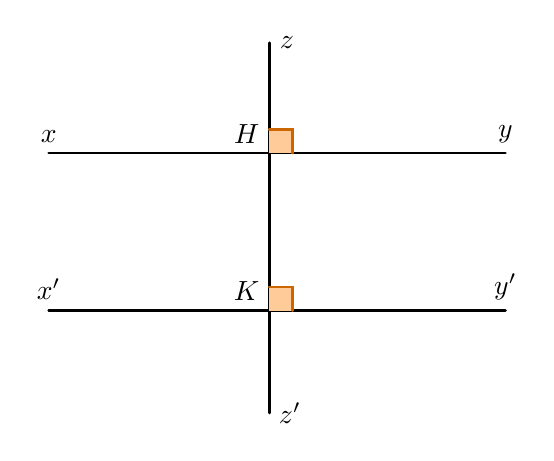
\begin{tikzpicture}[line cap=round]
\draw[line width=1pt] (0,-1.3) -- (0,3.4) node[right] {$z$};
\node[right] at (0,-1.3) {$z'$};
\draw[line width=1pt] (-2.8,2) node[above] {$x$} -- (3,2) node[above] {$y$};
\draw[line width=1pt] (-2.8,0) node[above] {$x'$} -- (3,0) node[above] {$y'$};
\fill[orange!40] (0,2) rectangle (0.3,2.3); \fill[orange!40] (0,0) rectangle (0.3,0.3);
\draw[orange!80!black, line width=1pt] (0.3,2) -- (0.3,2.3) -- (0,2.3); \draw[orange!80!black, line width=1pt] (0.3,0) -- (0.3,0.3) -- (0,0.3);
\node[above left] at (0,2) {$H$}; \node[above left] at (0,0) {$K$};
\end{tikzpicture}}
\nhanxet{Cùng vuông góc thì song song}{Hai đường thẳng phân biệt cùng vuông góc với một đường thẳng thứ ba thì \textbf{song song} với nhau. \\ $xy\perp zz'$, $x'y'\perp zz'$ $\Rightarrow$ $xy\parallel x'y'$.}

\cherry{Một câu nữa nhé!}
\hinhrieng{\begin{hinhbuoc}
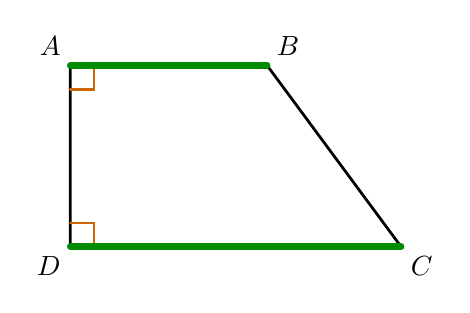
\begin{tikzpicture}[line cap=round]
\coordinate (A) at (0,2.3); \coordinate (B) at (2.5,2.3); \coordinate (C) at (4.2,0); \coordinate (D) at (0,0);
\draw[line width=1pt] (A) -- (B) -- (C) -- (D) -- cycle;
\draw[orange!80!black, line width=1pt] (0.3,2.3) -- (0.3,2.0) -- (0,2.0);
\draw[orange!80!black, line width=1pt] (0.3,0) -- (0.3,0.3) -- (0,0.3);
\hien{2}{\draw[green!55!black, line width=2.4pt] (A) -- (B); \draw[green!55!black, line width=2.4pt] (D) -- (C);}
\node[above left] at (A) {$A$}; \node[above right] at (B) {$B$}; \node[below right] at (C) {$C$}; \node[below left] at (D) {$D$};
\end{tikzpicture}
\loibuoc{Tứ giác $ABCD$ có góc $A$ và góc $D$ vuông.}
\loibuoc{$AB\parallel DC$.}
\end{hinhbuoc}}
\thungay{Tứ giác $ABCD$ có góc $A$ và góc $D$ vuông. Vì sao $AB\parallel DC$?}{Vì $AB$ và $DC$ cùng vuông góc với $AD$}{Vì $AB=DC$}{Đúng! Hai đường thẳng phân biệt cùng vuông góc với một đường thẳng thứ ba thì song song.}{$AB$ và $DC$ không bằng nhau. Lí do là chúng cùng vuông góc với $AD$.}

% ---------------- PHẦN 4 ----------------
\phan{Vẽ hai đường thẳng song song}{Vẽ bằng ê ke và giải thích vì sao}
\nhaclai{Dùng góc $60^\circ$ của ê ke tạo ra hai góc đồng vị cùng bằng $60^\circ$ ở $A$ và $B$, nên $b\parallel a$.}
\hinhchung{\begin{hinhbuoc}
\begin{tikzpicture}[line cap=round]
\coordinate (A) at (3.2,2.2); \coordinate (B) at (1.9298,0);
\draw[line width=1pt] (-0.3,0) -- (6.2,0) node[above] {$a$};
\phu{2}{2}{\draw[orange!80!black, fill=orange!30, line width=1pt] (B) -- ++(1.6,0) -- ++(0,2.7713) -- cycle;}
\hien{3}{\draw[line width=1pt] ($(B)+(240:0.9)$) -- ($(A)+(60:1.7)$);}
\phu{4}{4}{\draw[orange!80!black, fill=orange!30, line width=1pt] (A) -- ++(1.6,0) -- ++(0,2.7713) -- cycle;}
\hien{5}{\draw[red, line width=1.5pt] (-0.3,2.2) -- (6.2,2.2) node[above] {$b$};
\fill[orange!50] (A) -- ++(0:0.55) arc (0:60:0.55) -- cycle; \fill[orange!50] (B) -- ++(0:0.55) arc (0:60:0.55) -- cycle;
\node[font=\small\bfseries, text=orange!80!black] at ($(A)+(30:0.9)$) {$60^\circ$}; \node[font=\small\bfseries, text=orange!80!black] at ($(B)+(30:0.9)$) {$60^\circ$};}
\hien{2}{\fill (B) circle (0.07); \node[below left] at (B) {$B$};}
\fill (A) circle (0.07); \node[above left] at (A) {$A$};
\path (-0.6,-0.6) rectangle (6.4,5.1);
\end{tikzpicture}
\loibuoc{Cho đường thẳng $a$ và điểm $A$ nằm ngoài $a$.}
\loibuoc{Đặt ê ke sao cho góc $60^\circ$ có một cạnh nằm trên $a$, cạnh kia đi qua $A$. Đỉnh của góc $60^\circ$ là $B$.}
\loibuoc{Vẽ đường thẳng đi qua $A$ và $B$.}
\loibuoc{Đặt ê ke để góc $60^\circ$ có đỉnh $A$, một cạnh nằm trên đường thẳng $AB$ (giống như ở $B$).}
\loibuoc{Vẽ đường thẳng $b$ theo cạnh còn lại của ê ke.}
\end{hinhbuoc}}

\cherry{Cùng vẽ đường thẳng $b$ qua $A$ và song song với $a$, bằng góc $60^\circ$ của ê ke.}
\xemtungbuoc

\cherry{Vì sao cách vẽ này đúng?}
\trangthai{buoc=5}
\thungay{Vì sao đường thẳng $b$ vừa vẽ song song với $a$?}{Hai góc $60^\circ$ ở $A$ và $B$ là hai góc đồng vị bằng nhau}{Vì $b$ đi qua điểm $A$ nằm ngoài $a$}{Chính xác! Đó là dấu hiệu nhận biết hai đường thẳng song song.}{Đi qua $A$ chưa đủ. Lí do là hai góc đồng vị ở $A$ và $B$ cùng bằng $60^\circ$.}

% ---------------- KẾT BÀI ----------------
\begin{ketbai}
\cherry{Quay lại câu hỏi của người thợ. Giờ em trả lời được rồi!}
\hinhrieng{\begin{hinhbuoc}
\begin{tikzpicture}[line cap=round]
\fill[orange!12] (-3.2,0) -- (0,4) -- (3.2,0) -- cycle;
\draw[brown!70!black, line width=3pt, line join=round] (-3.2,0) -- (0,4) -- (3.2,0);
\fill[brown!70!black] (-3.3,-0.35) rectangle (3.3,0);
\draw[brown!80!black, line width=3.5pt] (-2.5,0.9) -- (2.5,0.9);
\draw[brown!80!black, line width=3.5pt] (-1.75,1.9) -- (1.75,1.9);
\draw[brown!80!black, line width=3.5pt] (-1,2.9) -- (1,2.9);
\draw[brown!60!black, line width=4pt] (0,0.05) -- (0,3.9);
\node[font=\small, text=brown!50!black, right] at (0.1,3.55) {thanh dọc};
\draw[red, line width=1.2pt] (0.3,0.9) -- (0.3,1.2) -- (0,1.2);
\draw[red, line width=1.2pt] (0.3,1.9) -- (0.3,2.2) -- (0,2.2);
\draw[red, line width=1.2pt] (0.3,2.9) -- (0.3,3.2) -- (0,3.2);
\hien{2}{\fill[orange, opacity=0.45] (0,0.9) -- (0.5,0.9) arc (0:90:0.5) -- cycle;
\fill[orange, opacity=0.45] (0,1.9) -- (0.5,1.9) arc (0:90:0.5) -- cycle;
\fill[orange, opacity=0.45] (0,2.9) -- (0.5,2.9) arc (0:90:0.5) -- cycle;}
\end{tikzpicture}
\loibuoc{Các thanh ngang đều vuông góc với thanh dọc.}
\loibuoc{Các góc tô cam là các góc đồng vị, cùng bằng $90^\circ$.}
\end{hinhbuoc}}
\thungay{Vì sao các thanh ngang song song với nhau?}{Vì chúng cùng vuông góc với thanh dọc}{Vì các thanh ngang được cưa dài bằng nhau}{Đúng! Thanh dọc cắt các thanh ngang tạo các góc đồng vị cùng bằng $90^\circ$. Hai đường thẳng phân biệt cùng vuông góc với một đường thẳng thứ ba thì song song.}{Độ dài không quyết định. Lí do là chúng cùng vuông góc với thanh dọc, tạo các góc đồng vị cùng bằng $90^\circ$.}
\emdahoc{Nhận biết cặp góc so le trong, cặp góc đồng vị.}{Có một cặp so le trong bằng nhau thì cặp còn lại và các cặp đồng vị bằng nhau.}{Dấu hiệu: một cặp so le trong hoặc đồng vị bằng nhau thì hai đường thẳng song song.}{Vẽ đường thẳng song song bằng ê ke.}
\end{ketbai}

\end{lythuyet}
